\documentclass[11pt]{article}
\usepackage[margin=1in]{geometry}
\usepackage{booktabs}
\usepackage{graphicx}
\usepackage{array}
\usepackage{float}
\begin{document}
\section*{Step 10 Final Robustness Report}
This report implements the final participant-fixed-effects robustness check using the same Step~9 duration-aware front ROI outcome and the same included cohort, with 36 participant-sessions, 30 questions, and 1075 trials.
The primary inferential specification used Two-way cluster (participant + question).
\subsection*{Primary Model}
\begin{tabular}{p{0.42\linewidth}p{0.50\linewidth}}
\toprule
Metric & Value\\
\midrule
Robust SE type & Two-way cluster (participant + question)\\
Included participants & 36\\
Included questions & 30\\
Included trials & 1075\\
Condition beta & 3.016e-08\\
Condition SE & 2.351e-08\\
Condition test statistic & 1.283\\
Condition p-value & 0.209749\\
Condition 95\% CI & [-1.793e-08, 7.824e-08]\\
Global block-order beta & 4.422e-09\\
Within-block-position beta & -6.034e-09\\
Word-count beta & -4.611e-08\\
ENEM-correctness beta & 3.251e-09\\
\bottomrule
\end{tabular}

\begin{figure}[H]
\centering
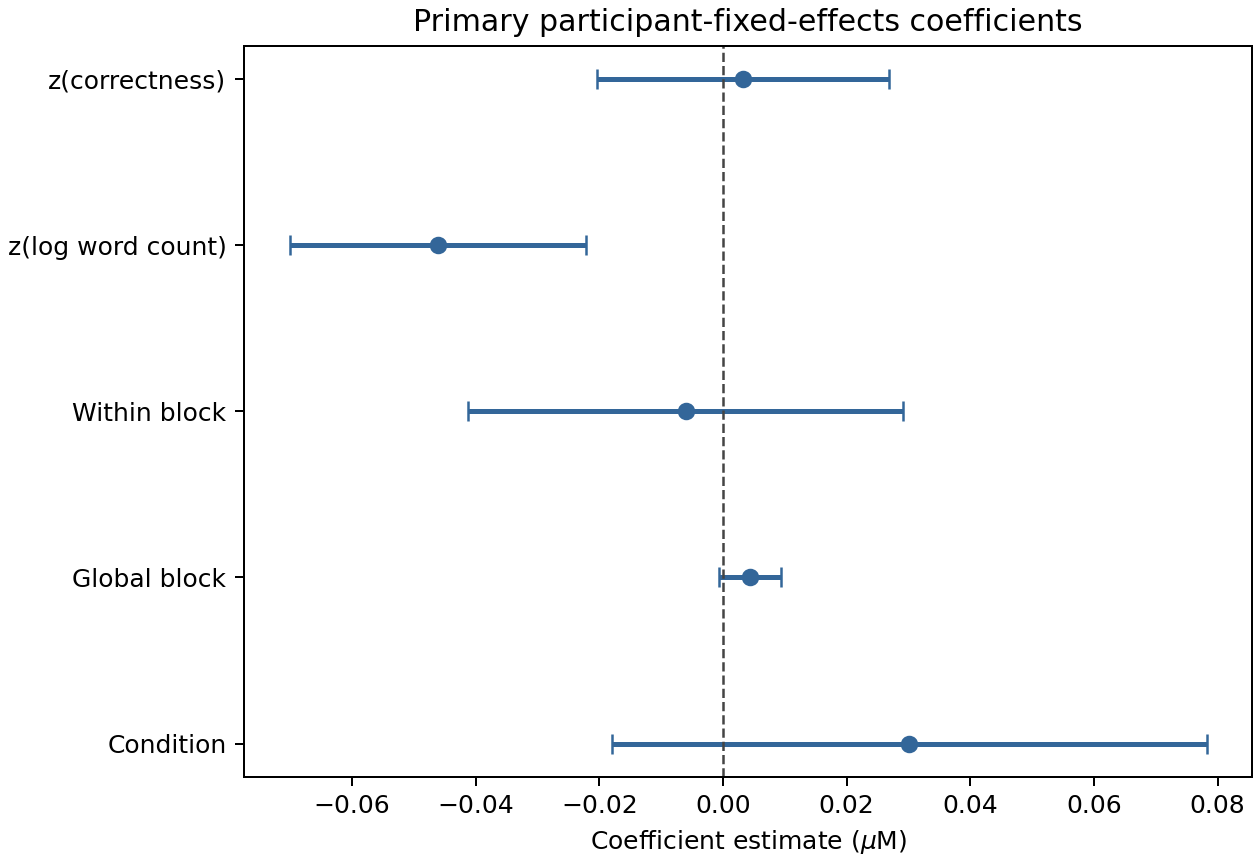
\includegraphics[width=0.78\linewidth]{../../figures/step10/primary_condition_coefficient_plot.png}
\caption{Coefficient plot for the primary participant-fixed-effects model.}
\end{figure}
\subsection*{Sensitivity Models}
\begin{tabular}{p{0.28\linewidth}p{0.20\linewidth}p{0.20\linewidth}p{0.10\linewidth}p{0.08\linewidth}p{0.12\linewidth}}
\toprule
Model & SE type & Beta / range & SE & p & 95% CI\\
\midrule
Primary participant-fixed-effects model & Two-way cluster (participant + question) & 3.016e-08 & 2.351e-08 & 0.209749 & [-1.793e-08, 7.824e-08]\\
Participant-clustered participant-fixed-effects model & Participant-clustered & 3.016e-08 & 2.058e-08 & 0.151850 & [-1.163e-08, 7.194e-08]\\
Question-clustered participant-fixed-effects model & Question-clustered & 3.016e-08 & 2.449e-08 & 0.228028 & [-1.993e-08, 8.024e-08]\\
HC3 participant-fixed-effects model & HC3 heteroskedasticity-robust & 3.016e-08 & 2.212e-08 & 0.173034 & [-1.324e-08, 7.356e-08]\\
Fixed-window front ROI benchmark under participant fixed effects & Two-way cluster (participant + question) & 2.235e-08 & 1.780e-08 & 0.219180 & [-1.405e-08, 5.874e-08]\\
No-override participant-fixed-effects model & Two-way cluster (participant + question) & 1.910e-08 & 2.086e-08 & 0.367415 & [-2.357e-08, 6.178e-08]\\
Back ROI benchmark under participant fixed effects & Two-way cluster (participant + question) & 1.388e-08 & 1.119e-08 & 0.224774 & [-9.009e-09, 3.678e-08]\\
Leave-one-question-out range & Primary robust SE & 1.885e-08 to 4.181e-08; p range 0.079410 to 0.412718 &  &  & \\
Leave-one-participant-out range & Primary robust SE & 2.196e-08 to 4.119e-08; p range 0.067180 to 0.292688 &  &  & \\
\bottomrule
\end{tabular}

\begin{figure}[H]
\centering
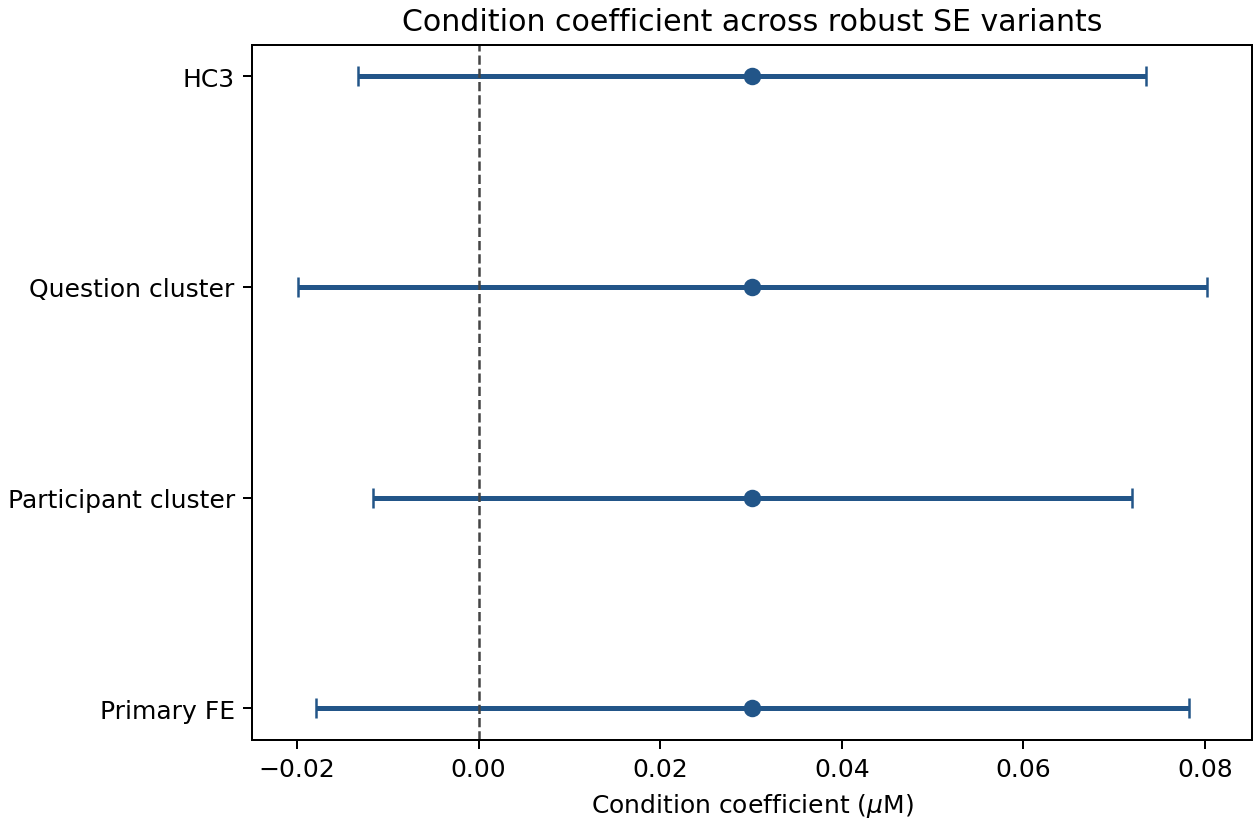
\includegraphics[width=0.78\linewidth]{../../figures/step10/robust_se_comparison.png}
\caption{Condition coefficient under the robust standard-error variants.}
\end{figure}
\begin{figure}[H]
\centering
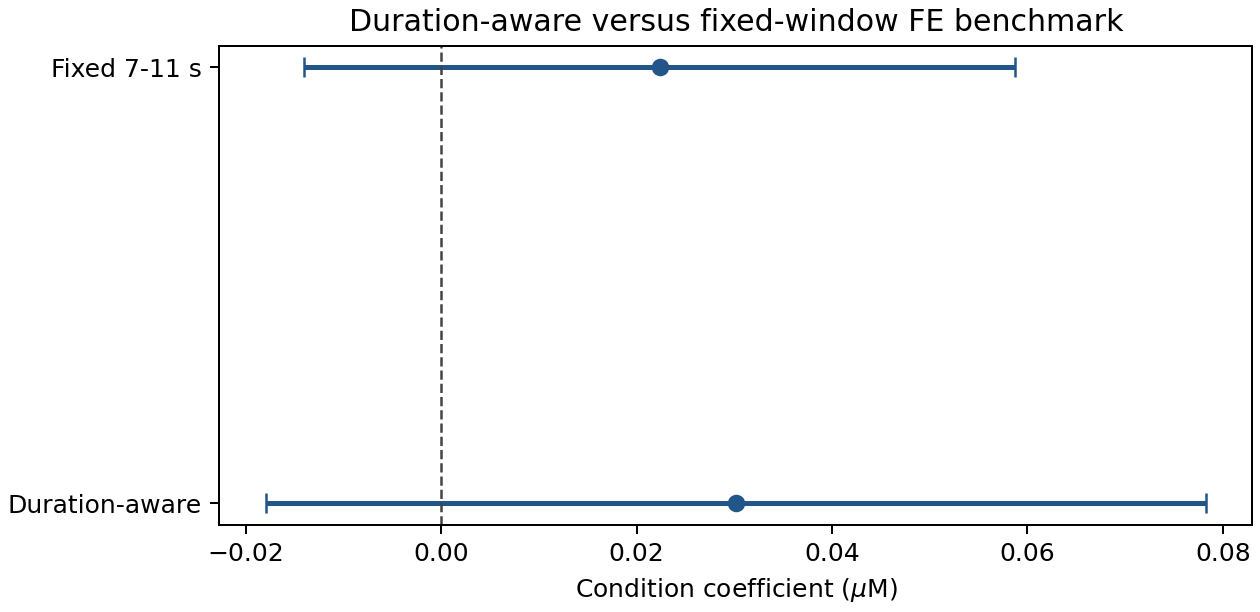
\includegraphics[width=0.78\linewidth]{../../figures/step10/fixed_vs_variable_fe_benchmark.png}
\caption{Final fixed-window versus duration-aware benchmark under participant fixed effects.}
\end{figure}
\begin{figure}[H]
\centering
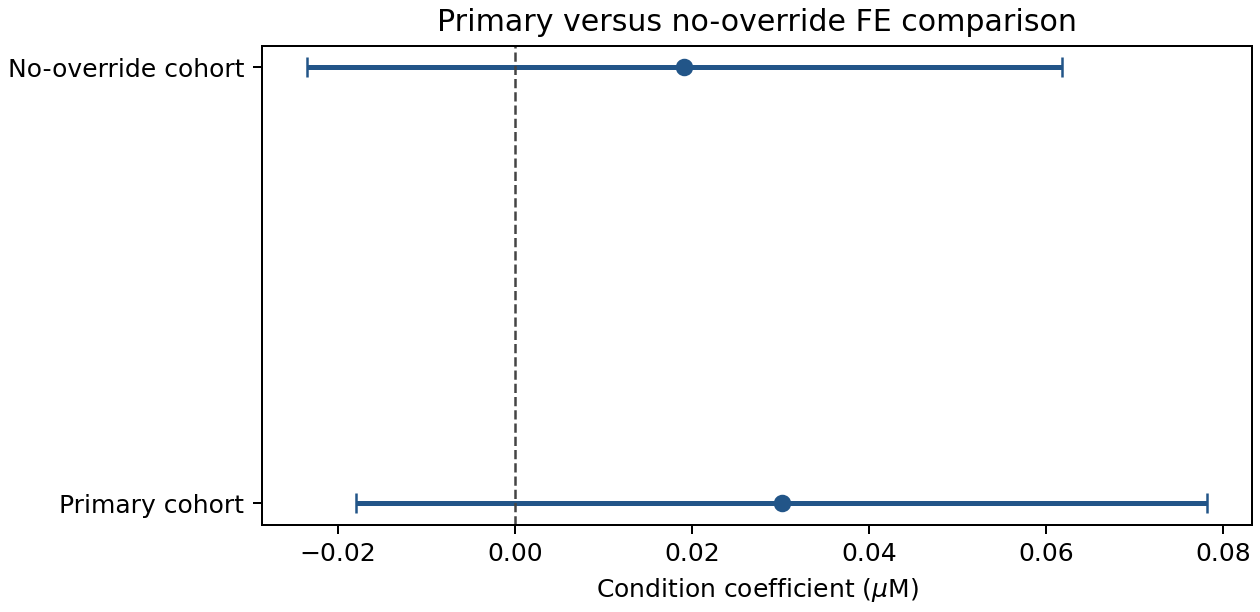
\includegraphics[width=0.78\linewidth]{../../figures/step10/no_override_comparison.png}
\caption{Primary cohort versus no-override sensitivity comparison.}
\end{figure}
\begin{figure}[H]
\centering
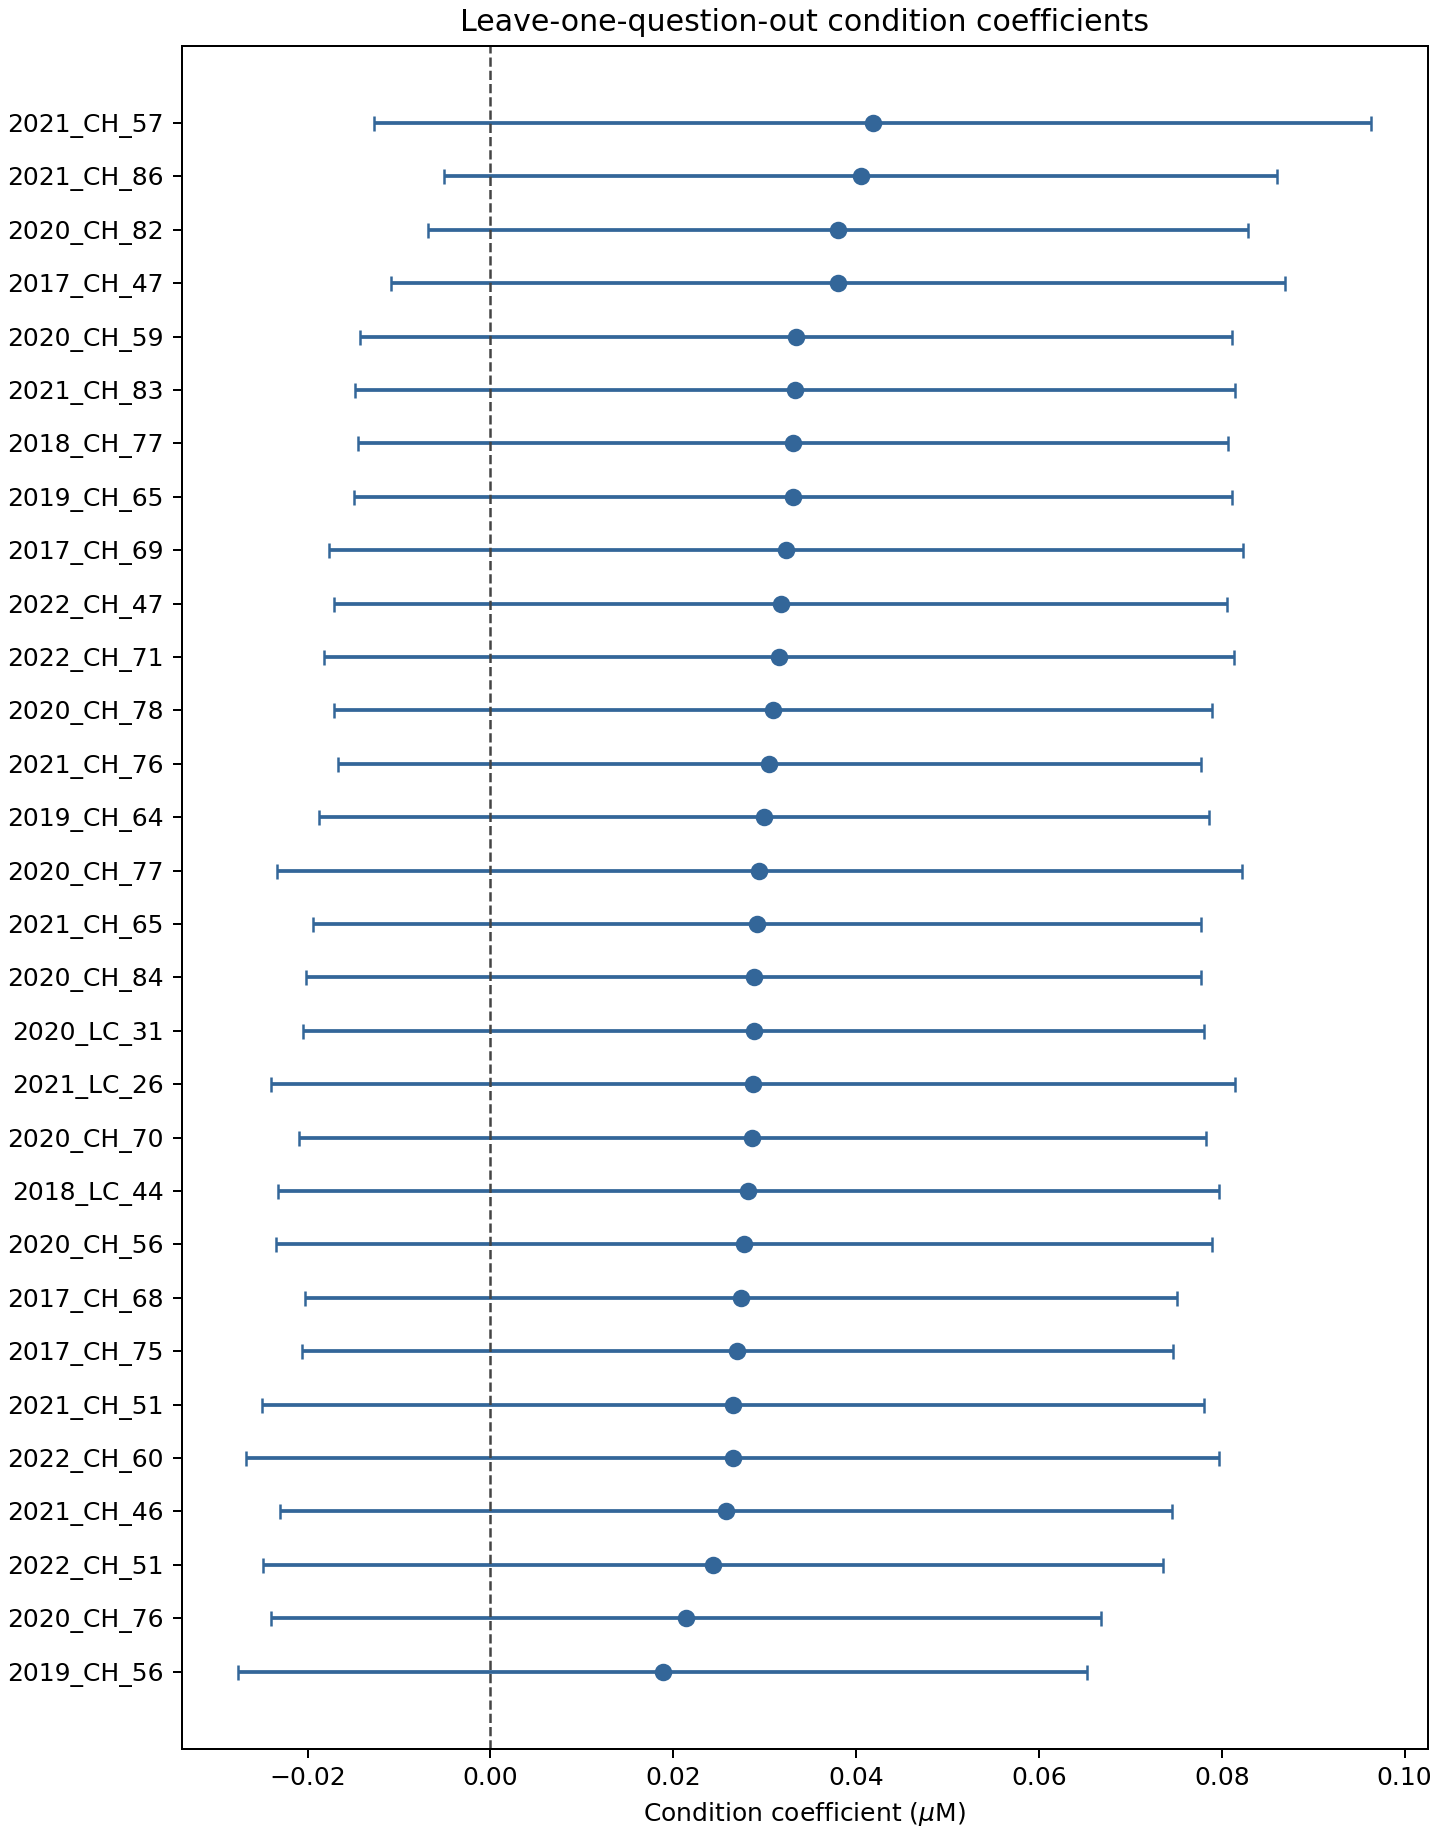
\includegraphics[width=0.82\linewidth]{../../figures/step10/leave_one_question_out_plot.png}
\caption{Leave-one-question-out condition coefficients with 95\% confidence intervals.}
\end{figure}
\begin{figure}[H]
\centering
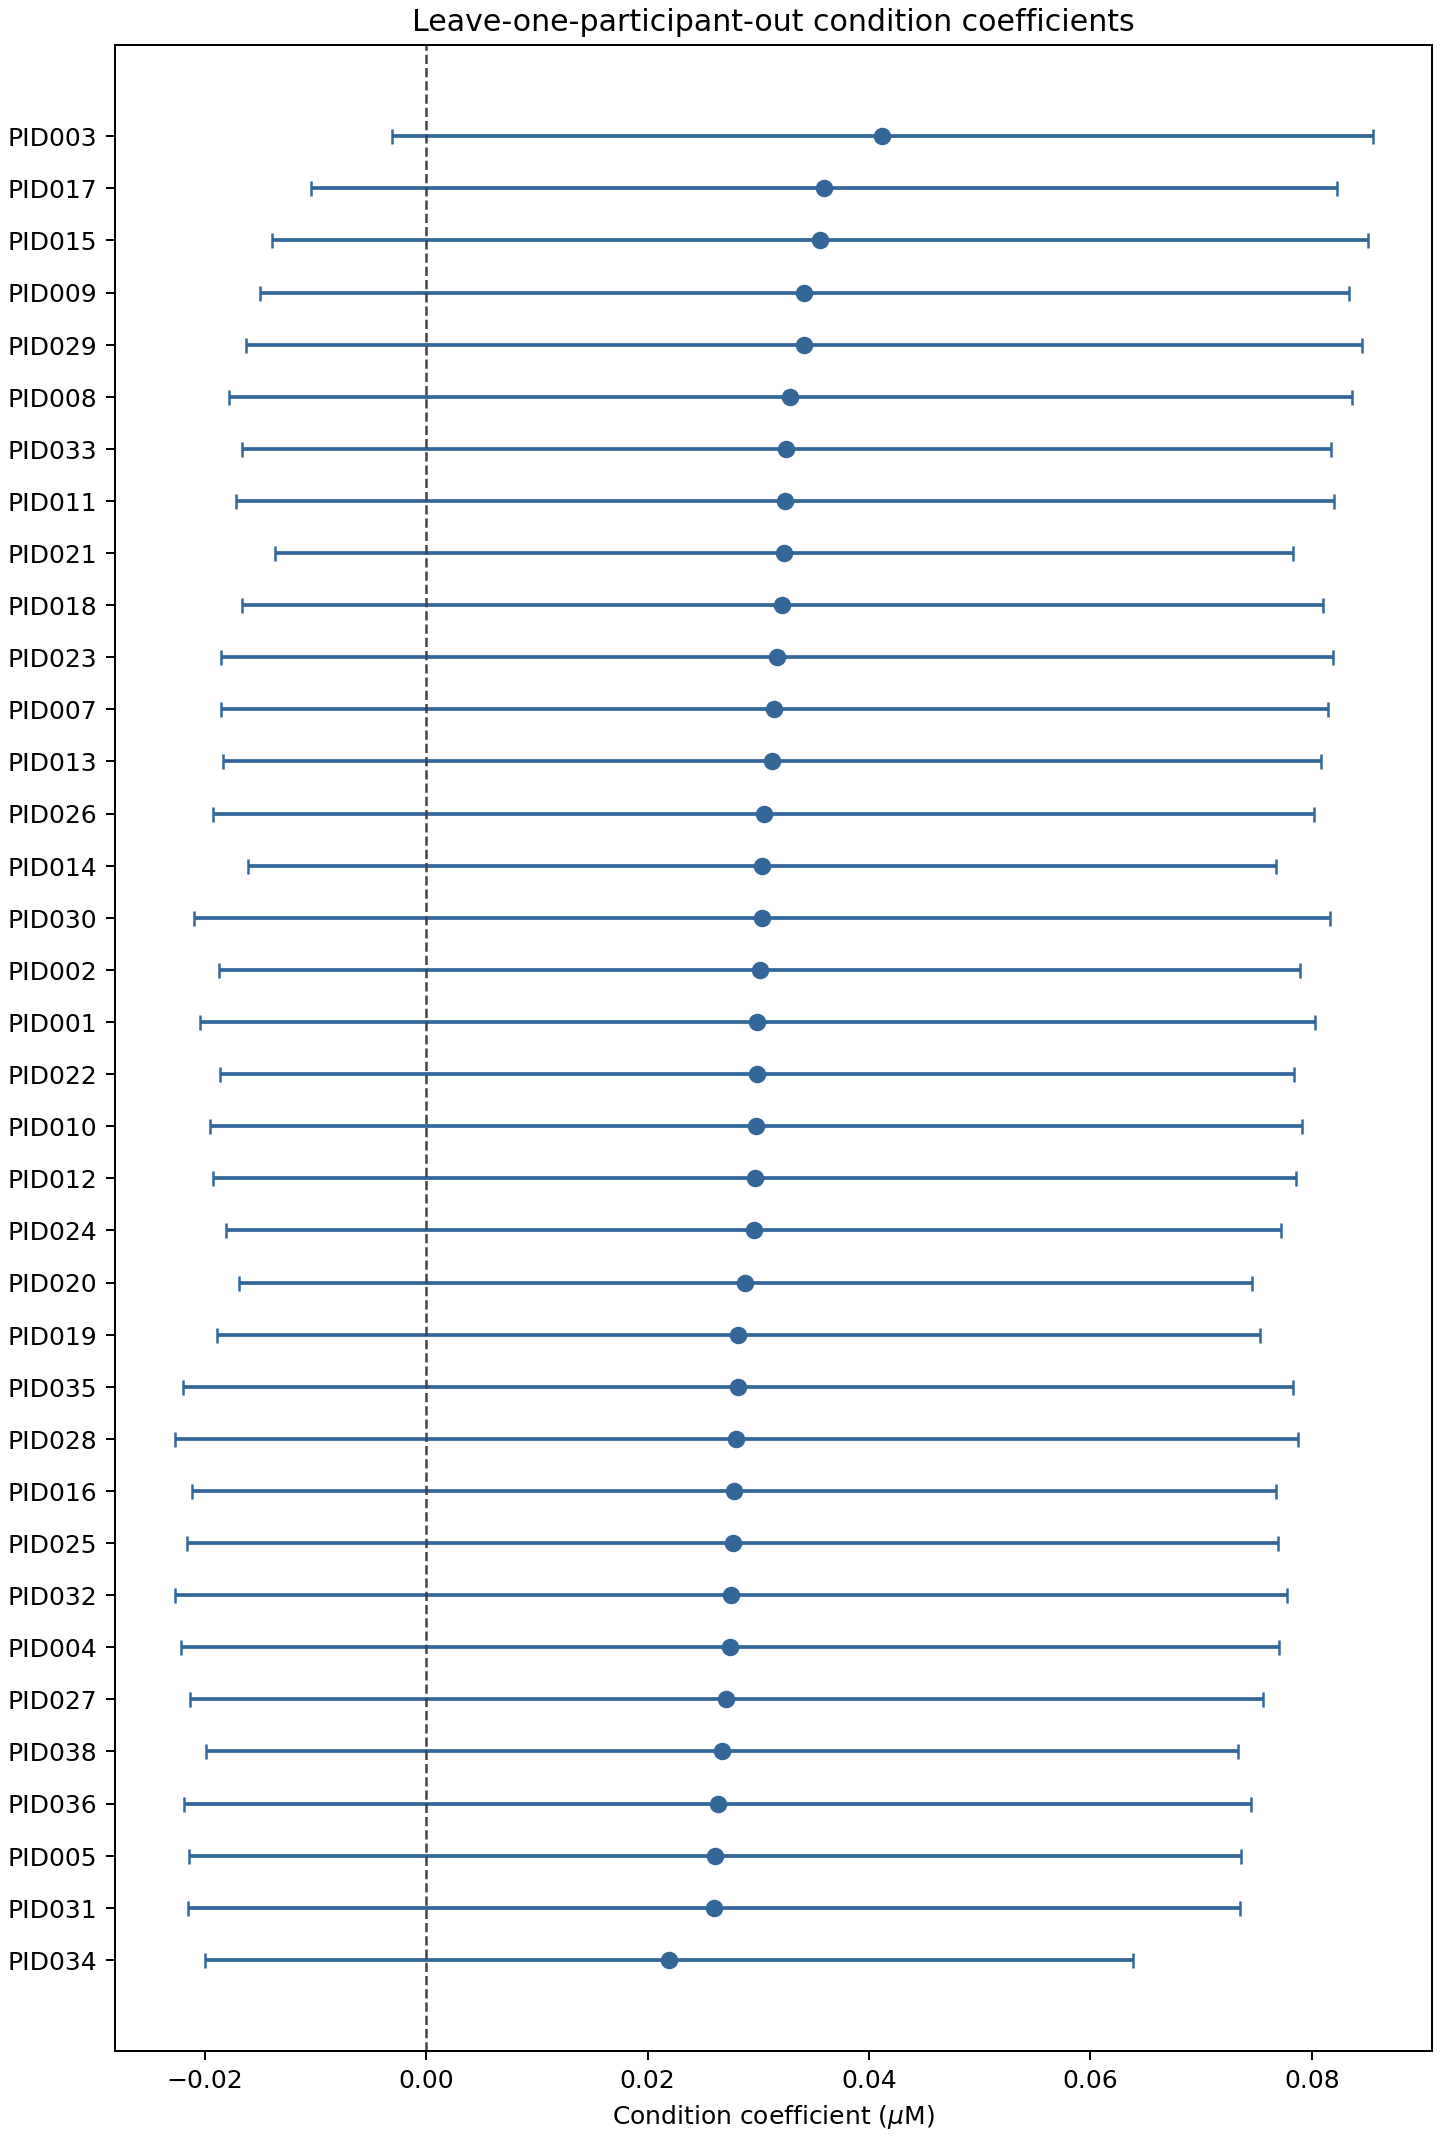
\includegraphics[width=0.82\linewidth]{../../figures/step10/leave_one_participant_out_plot.png}
\caption{Leave-one-participant-out condition coefficients with 95\% confidence intervals.}
\end{figure}
\subsection*{Warnings And Notes}
\begin{itemize}
\item No Step 10-specific warnings were generated.
\end{itemize}
\subsection*{Final Conclusion}
In the final participant-fixed-effects robustness analysis, the abstract-versus-concrete effect in the left frontal ROI was not statistically significant (beta=3.016e-08, SE=2.351e-08, p=0.209749, 95% CI [-1.793e-08, 7.824e-08]). Together with the non-significant sensitivity models, this suggests that the frontal condition tendency remains descriptive but does not receive robust statistical support in the current dataset.

\end{document}
